\documentclass[xetex,18pt,aspectratio=43]{beamer}

\usepackage{caption}
\usepackage[percent]{overpic}
\usepackage{xecyr}
\usepackage{xunicode}
\usepackage[absolute,overlay]{textpos}
\usepackage{fontspec}
\usepackage{calc}
\usepackage{multicol}
\usepackage{hyperref}
\usepackage{setspace}
\usepackage{tikz}
%\usepackage{coloremoji}
\usepackage{csquotes}
\usepackage[export]{adjustbox}
\usepackage[normalem]{ulem}
%\usepackage{cancel}
%\usepackage[texcoord,grid,gridunit=mm,gridcolor=red!10,subgridcolor=green!10]{eso-pic}
\defaultfontfeatures{Ligatures=TeX}
\setmainfont{Trebuchet MS}
\usepackage{polyglossia}
\setdefaultlanguage[spelling=modern]{russian}
\newfontfamily{\cyrillicfont}{Trebuchet MS}
\newfontfamily{\cyrillicfontsf}{Trebuchet MS}
\newfontfamily{\cyrillicfonttt}{Trebuchet MS}
\newfontface\lserif{Microsoft Sans Serif}

\newcommand\Bigfont{\fontsize{20}{20}\selectfont}
\newcommand\Authorfont{\fontsize{17}{17}\selectfont}
\newcommand\Orgfont{\fontsize{13}{13}\selectfont}

\definecolor{cadmiumgreen}{rgb}{0.0, 0.42, 0.24}
\definecolor{darkpastelgreen}{rgb}{0.01, 0.75, 0.24}
\definecolor{darkorange}{rgb}{1.0, 0.55, 0.0}
\definecolor{darkorchid}{rgb}{0.6, 0.2, 0.8}
\definecolor{darkpink}{rgb}{0.91, 0.33, 0.5}

\mode<presentation>
{
  %\usetheme{Boadilla}      % or try Darmstadt, Madrid, Warsaw, ...
  \usecolortheme{default} % or try albatross, beaver, crane, ...
  %\usefonttheme{default}  % or try serif, structurebold, ...
  \setbeamertemplate{navigation symbols}{}
  \setbeamertemplate{caption}[numbered]
  \setbeamertemplate{itemize items}[circle]
  \setbeamerfont{title}{series=\bfseries,parent=structure}
  \setbeamerfont{frametitle}{size=\huge}
} 

\makeatother
\setbeamertemplate{footline}
{
  \leavevmode%
  \hbox{%
  \begin{beamercolorbox}[wd=.35\paperwidth,ht=2.5ex,dp=1ex,center]{author in head/foot}%
    \usebeamerfont{author in head/foot}\insertshortauthor
  \end{beamercolorbox}%
  \begin{beamercolorbox}[wd=.65\paperwidth,ht=2.5ex,dp=1ex,center]{title in head/foot}%
    \usebeamerfont{title in head/foot}\insertshorttitle\hfill
    \insertframenumber{} / \inserttotalframenumber\hspace*{-8ex}
  \end{beamercolorbox}}%
  \vskip0pt%
}
\makeatletter

\title[Давайте инструментируем что-нибудь]{}
\author[Александр Чистяков, vdsina.ru]{}
\date{}

\begin{document}

{ % all template changes are local to this group.
    \setbeamertemplate{navigation symbols}{}
    %\setbeamertemplate{background}[grid][step=10]
    \setbeamertemplate{background}{
\includegraphics[width=\paperwidth,height=\paperheight,keepaspectratio]{img/firstslide.png}}
    \begin{frame}[plain]
      \setstretch{1.2}
      \begin{textblock*}{\framewidth}(0.95cm,3.0cm) % {block width} (coords)
        \Bigfont
          \begin{center}
          Давайте инструментируем что-нибудь
          \end{center}
      \end{textblock*}
      \begin{textblock*}{\framewidth}(0.95cm,5.8cm) % {block width} (coords)
        \Authorfont
          \begin{center}
          Александр Чистяков
          \end{center}
      \end{textblock*}
      \begin{textblock*}{\framewidth}(0.95cm,6.9cm) % {block width} (coords)
        \Orgfont
          \begin{center}
          \href{https://vdsina.ru}{\color{blue}vdsina.ru}, евангелист
          \end{center}
      \end{textblock*}
     \end{frame}
}


\begin{Large}

\begin{frame}{\ \ \ Очень краткое содержание}
\setstretch{1.2}
\begin{textblock*}{\framewidth-0.8cm}(0.5cm,1.5cm)
\begin{itemize}
  \item Давайте инструментируем
\end{itemize}
\end{textblock*}
\end{frame}

\begin{frame}{\ \ \ Очень краткое содержание}
\setstretch{1.2}
\begin{textblock*}{\framewidth-0.8cm}(0.5cm,1.5cm)
\begin{itemize}
  \item Давайте инструментируем
  \item Что-нибудь
\end{itemize}
\end{textblock*}
\end{frame}

\begin{frame}{\ \ \ Приложение на JavaScript?}
\setstretch{1.2}
\begin{textblock*}{\framewidth-0.8cm}(0.5cm,1.5cm)
\begin{itemize}
  \item Используем пакет prom-client
\end{itemize}
\begin{minipage}{\textwidth}
  \centering
  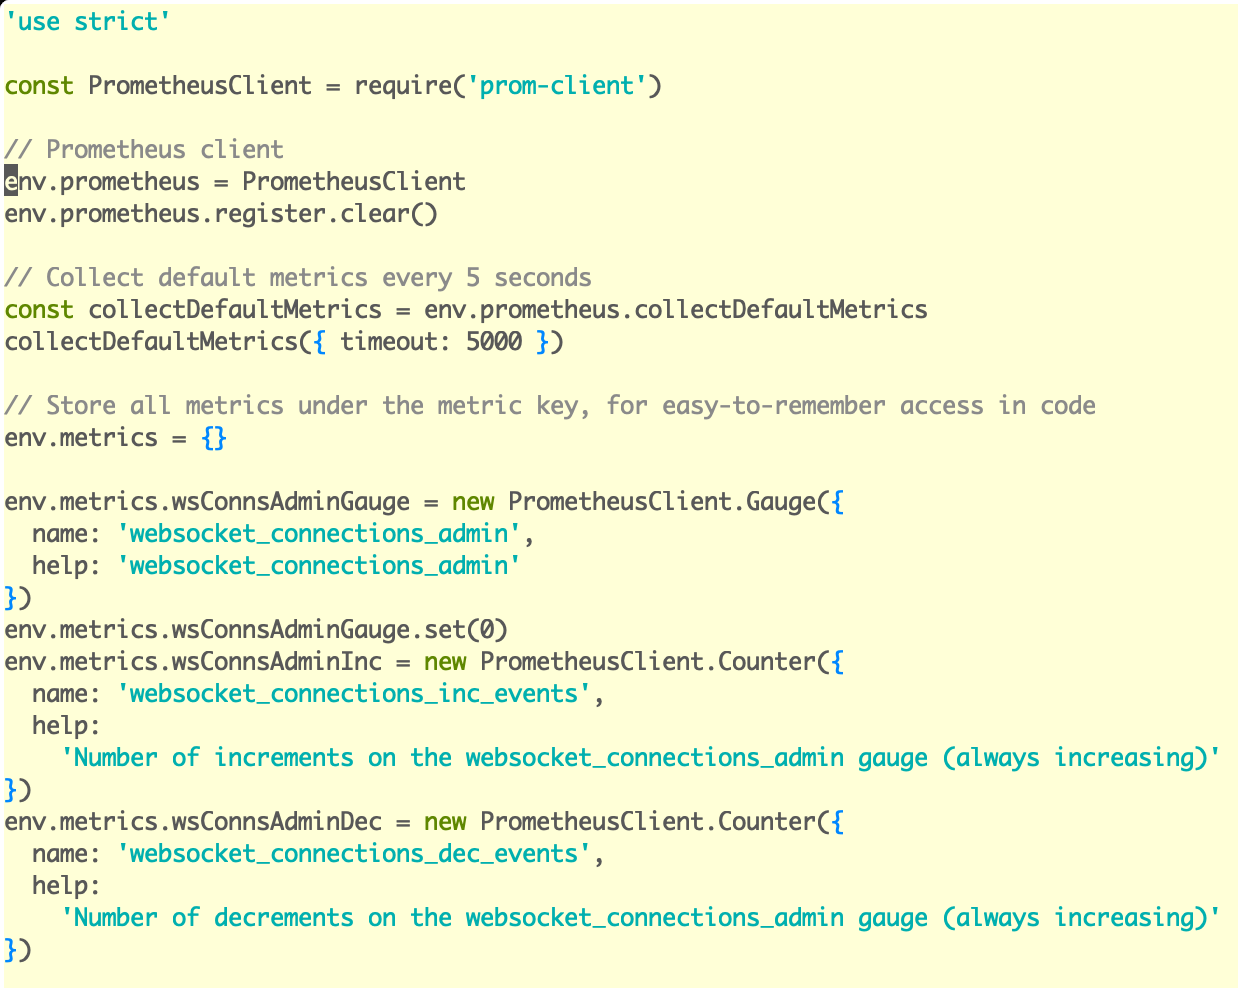
\includegraphics[height=6.9cm]{img/javascript}
\end{minipage}
\end{textblock*}
\end{frame}

\begin{frame}{\ \ \ Выглядит не очень сложно!}
\setstretch{1.2}
\begin{textblock*}{\framewidth-0.8cm}(0.5cm,1.5cm)
\begin{itemize}
  \item Давайте лучше инструментируем MongoDB
\end{itemize}
\end{textblock*}
\end{frame}

\begin{frame}{\ \ \ MongoDB}
\setstretch{1.2}
\begin{textblock*}{\framewidth-0.8cm}(0.5cm,1.5cm)
\begin{itemize}
  \item Написана на языке C++
\end{itemize}
\end{textblock*}
\end{frame}

\begin{frame}{\ \ \ MongoDB}
\setstretch{1.2}
\begin{textblock*}{\framewidth-0.8cm}(0.5cm,1.5cm)
\begin{itemize}
  \item Написана на языке C++
  \item Собирается при помощи SCons
\end{itemize}
\end{textblock*}
\end{frame}

\begin{frame}{\ \ \ Нам нужен план}
\setstretch{1.2}
\begin{textblock*}{\framewidth-0.8cm}(0.5cm,1.5cm)
\begin{itemize}
  \item Встроить дэшборд в MongoDB
\end{itemize}
\end{textblock*}
\end{frame}

\begin{frame}{\ \ \ Нам нужен план}
\setstretch{1.2}
\begin{textblock*}{\framewidth-0.8cm}(0.5cm,1.5cm)
\begin{itemize}
  \item Встроить дэшборд в MongoDB
  \item Видимо, написать дэшборд на C++?
\end{itemize}
\end{textblock*}
\end{frame}

\begin{frame}{\ \ \ Преимущества C++}
\setstretch{1.2}
\begin{textblock*}{\framewidth-0.8cm}(0.5cm,1.5cm)
\begin{itemize}
  \item Есть сегфолты
\end{itemize}
\end{textblock*}
\end{frame}

\begin{frame}{\ \ \ Преимущества C++}
\setstretch{1.2}
\begin{textblock*}{\framewidth-0.8cm}(0.5cm,1.5cm)
\begin{itemize}
  \item Есть сегфолты
  \item Можно прибавить к адресу в памяти число
\end{itemize}
\end{textblock*}
\end{frame}

\begin{frame}{\ \ \ Преимущества C++}
\setstretch{1.2}
\begin{textblock*}{\framewidth-0.8cm}(0.5cm,1.5cm)
\begin{itemize}
  \item Есть сегфолты
  \item Можно прибавить к адресу в памяти число
  \item Язык не слишком DevOps-friendly
\end{itemize}
\end{textblock*}
\end{frame}

\begin{frame}{\ \ \ Не будем брать C++}
\setstretch{1.2}
\begin{textblock*}{\framewidth-0.8cm}(0.5cm,1.5cm)
\begin{itemize}
  \item Встроим какой-нибудь другой язык
\end{itemize}
\end{textblock*}
\end{frame}

\begin{frame}{\ \ \ Не будем брать C++}
\setstretch{1.2}
\begin{textblock*}{\framewidth-0.8cm}(0.5cm,1.5cm)
\begin{itemize}
  \item Встроим какой-нибудь другой язык
  \item Lua?
\end{itemize}
\end{textblock*}
\end{frame}

\begin{frame}{\ \ \ Не будем брать C++}
\setstretch{1.2}
\begin{textblock*}{\framewidth-0.8cm}(0.5cm,1.5cm)
\begin{itemize}
  \item Встроим какой-нибудь другой язык
  \item Lua?
  \item GNU Guile?
\end{itemize}
\end{textblock*}
\end{frame}

\begin{frame}{\ \ \ Не будем брать C++}
\setstretch{1.2}
\begin{textblock*}{\framewidth-0.8cm}(0.5cm,1.5cm)
\begin{itemize}
  \item Встроим какой-нибудь другой язык
  \item Lua?
  \item GNU Guile?
  \item Nim
\end{itemize}
\end{textblock*}
\end{frame}

\begin{frame}{\ \ \ Преимущества Nim}
\setstretch{1.2}
\begin{textblock*}{\framewidth-0.8cm}(0.5cm,1.5cm)
\begin{itemize}
  \item Нет сегфолтов
\end{itemize}
\end{textblock*}
\end{frame}

\begin{frame}{\ \ \ Преимущества Nim}
\setstretch{1.2}
\begin{textblock*}{\framewidth-0.8cm}(0.5cm,1.5cm)
\begin{itemize}
  \item Нет сегфолтов
  \item Очень похож на Python
\end{itemize}
\end{textblock*}
\end{frame}

\begin{frame}{\ \ \ Преимущества Nim}
\setstretch{1.2}
\begin{textblock*}{\framewidth-0.8cm}(0.5cm,1.5cm)
\begin{itemize}
  \item Нет сегфолтов
  \item Очень похож на Python
  \item Строго и статически типизирован
\end{itemize}
\end{textblock*}
\end{frame}

\begin{frame}{\ \ \ Преимущества Nim}
\setstretch{1.2}
\begin{textblock*}{\framewidth-0.8cm}(0.5cm,1.5cm)
\begin{itemize}
  \item Нет сегфолтов
  \item Очень похож на Python
  \item Строго и статически типизирован
  \item Компилируется в код на C
\end{itemize}
\end{textblock*}
\end{frame}

\begin{frame}{\ \ \ Нам опять нужен план}
\setstretch{1.2}
\begin{textblock*}{\framewidth-0.8cm}(0.5cm,1.5cm)
\begin{itemize}
  \item Используем Nim для дэшборда и сбора метрик
\end{itemize}
\end{textblock*}
\end{frame}

\begin{frame}{\ \ \ Нам опять нужен план}
\setstretch{1.2}
\begin{textblock*}{\framewidth-0.8cm}(0.5cm,1.5cm)
\begin{itemize}
  \item Используем Nim для дэшборда и сбора метрик
  \item Компилируем Nim в C (.h + .a)
\end{itemize}
\end{textblock*}
\end{frame}

\begin{frame}{\ \ \ Нам опять нужен план}
\setstretch{1.2}
\begin{textblock*}{\framewidth-0.8cm}(0.5cm,1.5cm)
\begin{itemize}
  \item Используем Nim для дэшборда и сбора метрик
  \item Компилируем Nim в C (.h + .a)
  \item Собираем mongod при помощи SCons, используя полученные файлы
\end{itemize}
\end{textblock*}
\end{frame}

\begin{frame}{\ \ \ Реализация бриджа из C в Nim}
\setstretch{1.2}
\begin{textblock*}{\framewidth-0.8cm}(0.5cm,1.5cm)
\begin{itemize}
  \item startJesterP запускается в отдельном потоке
\end{itemize}
\begin{minipage}{\textwidth}
  \centering
  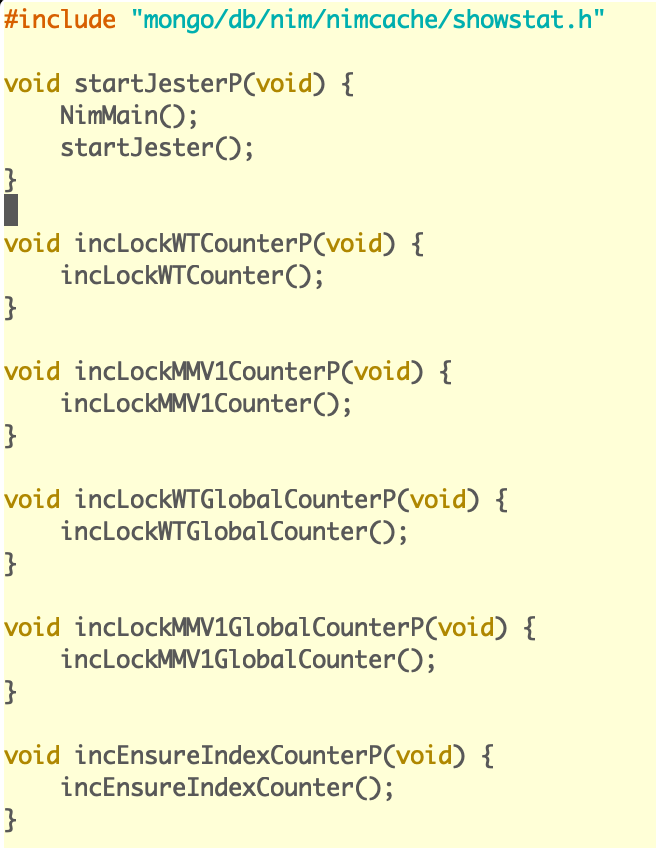
\includegraphics[height=6.1cm]{img/c}
\end{minipage}
\end{textblock*}
\end{frame}

\begin{frame}{\ \ \ Как ускорить сборку}
\setstretch{1.2}
\begin{textblock*}{\framewidth-0.8cm}(0.5cm,1.5cm)
\begin{itemize}
  \item scons --disable-warnings-as-errors {\bf -j80}
\end{itemize}
\end{textblock*}
\end{frame}

\begin{frame}{\ \ \ Это, вообще, законно?}
\setstretch{1.2}
\begin{textblock*}{\framewidth-0.8cm}(0.5cm,1.5cm)
\begin{itemize}
  \item Выглядит потокобезопасно
\end{itemize}
\begin{minipage}{\textwidth}
  \centering
  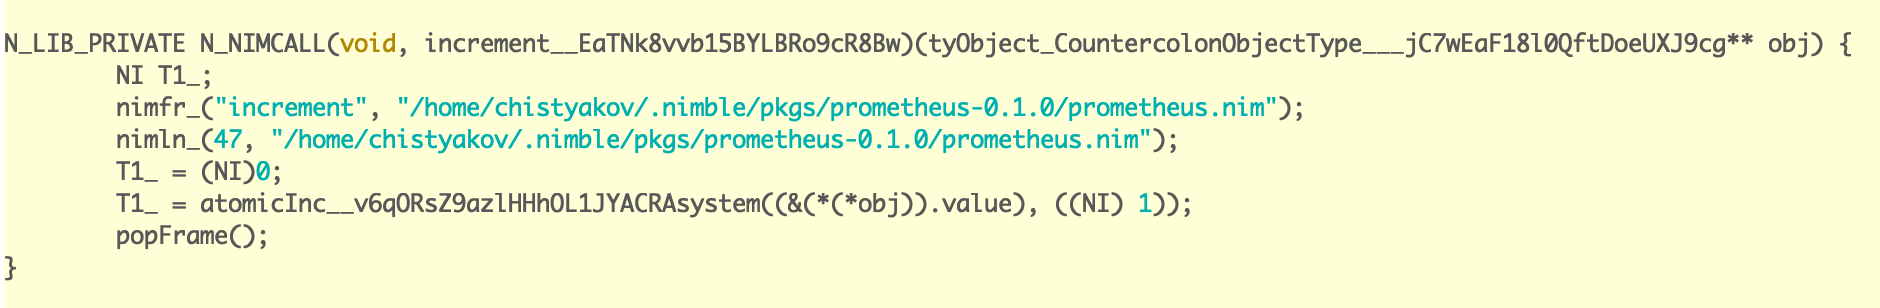
\includegraphics[height=3.1cm]{img/gencode1}
\end{minipage}
\end{textblock*}
\end{frame}

\begin{frame}{\ \ \ Это, вообще, законно?}
\setstretch{1.2}
\begin{textblock*}{\framewidth-0.8cm}(0.5cm,1.5cm)
\begin{itemize}
  \item Выглядит потокобезопасно
\end{itemize}
\begin{minipage}{\textwidth}
  \centering
  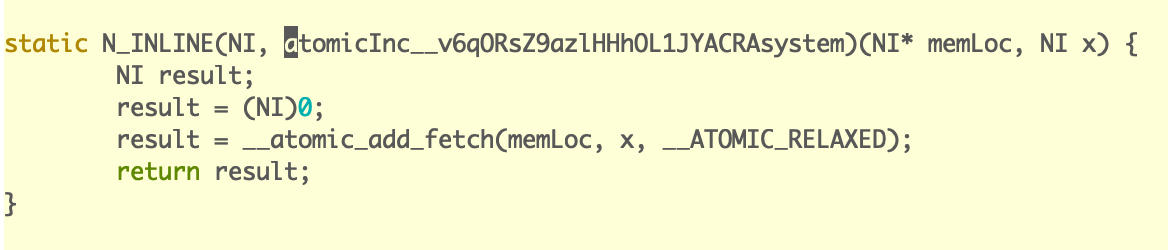
\includegraphics[height=3.1cm]{img/gencode2}
\end{minipage}
\end{textblock*}
\end{frame}

\begin{frame}{\ \ \  Это, вообще, работает?}
\setstretch{1.2}
\begin{textblock*}{\framewidth-0.8cm}(0.5cm,1.5cm)
\begin{itemize}
  \item Виден запуск Jester среди логгинга mongod
\end{itemize}
\begin{minipage}{\textwidth}
  \centering
  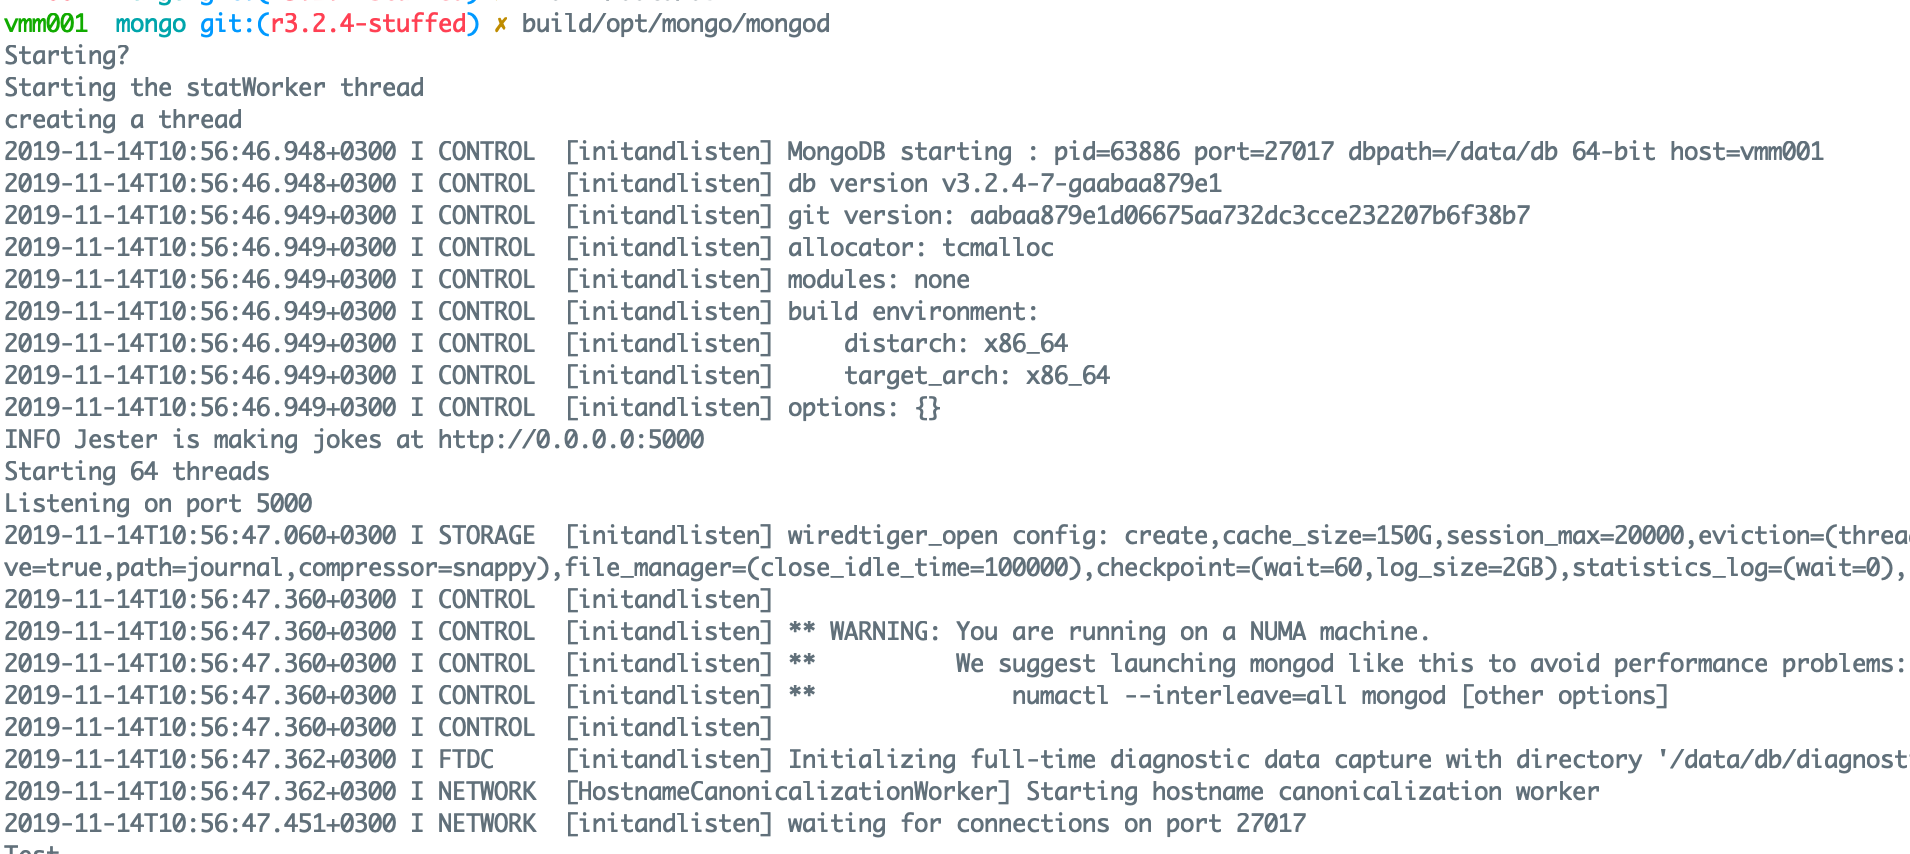
\includegraphics[height=5.8cm]{img/start}
\end{minipage}
\end{textblock*}
\end{frame}

\begin{frame}{\ \ \  Как все это выглядит?}
\setstretch{1.2}
\begin{textblock*}{\framewidth-0.8cm}(0.5cm,1.5cm)
\begin{itemize}
  \item Обычный дэшборд, только внутри mongod
\end{itemize}
\begin{minipage}{\textwidth}
  \centering
  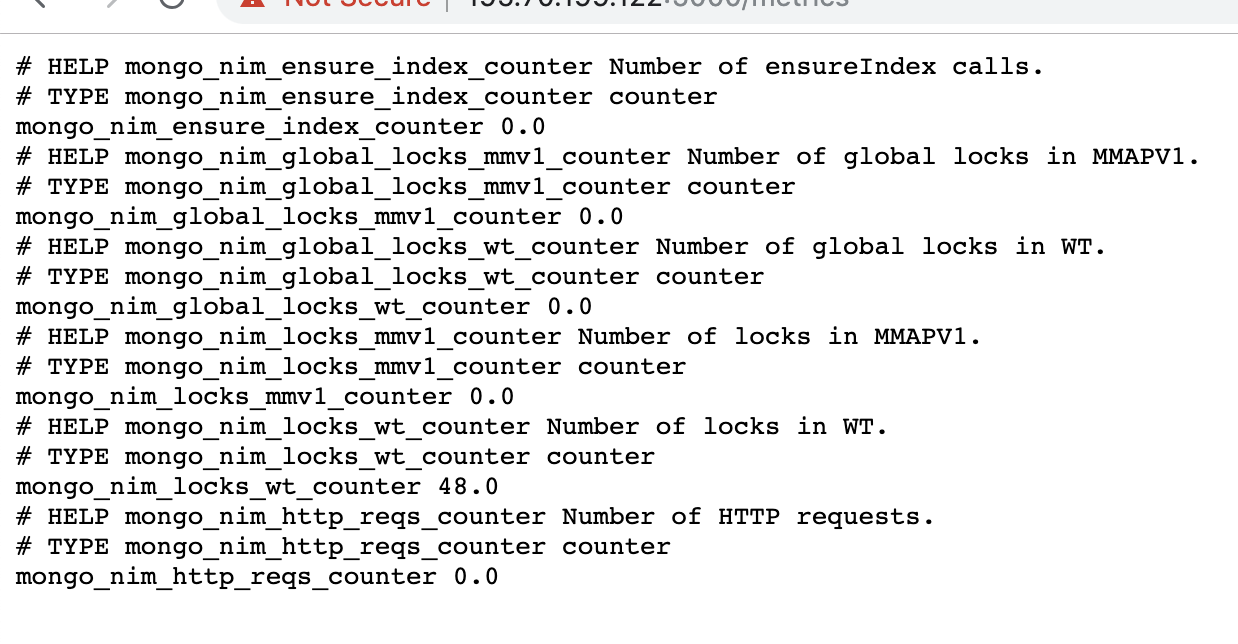
\includegraphics[height=6.1cm]{img/dashboard}
\end{minipage}
\end{textblock*}
\end{frame}

\begin{frame}{\ \ \ Выводы}
\setstretch{1.2}
\begin{textblock*}{\framewidth-0.8cm}(0.5cm,1.5cm)
\begin{itemize}
  \item Можно инструментировать что угодно
  \item Даже JavaScript
\end{itemize}
\end{textblock*}
\end{frame}

\begin{frame}{\ \ \ That's all, folks!}
\setstretch{1.2}
\begin{textblock*}{\framewidth-0.8cm}(0.5cm,1.5cm)
\begin{itemize}
  \item \href{mailto:alexclear@gmail.com}{\color{blue}{alexclear@gmail.com}}
  \item \href{https://telegram.me/lhommequipleure}{\color{blue}{https://telegram.me/lhommequipleure}}
  \item \href{https://telegram.me/demeliorator\_pod}{\color{blue}{https://telegram.me/demeliorator\_pod}}
\end{itemize}
\end{textblock*}
\end{frame}

\end{Large}

\end{document}
